\section[Chaine de numérisation]{La chaîne de numérisation : flux, traitements et archivage}
Une fois ces choix éditoriaux et ces corpus scientifiques stabilisés, l’enjeu pour la Bibliothèque Cujas a été de structurer une chaîne de production industrielle capable de matérialiser ces ambitions documentaires.

	\begin{figure}[htbp]
		\centering
		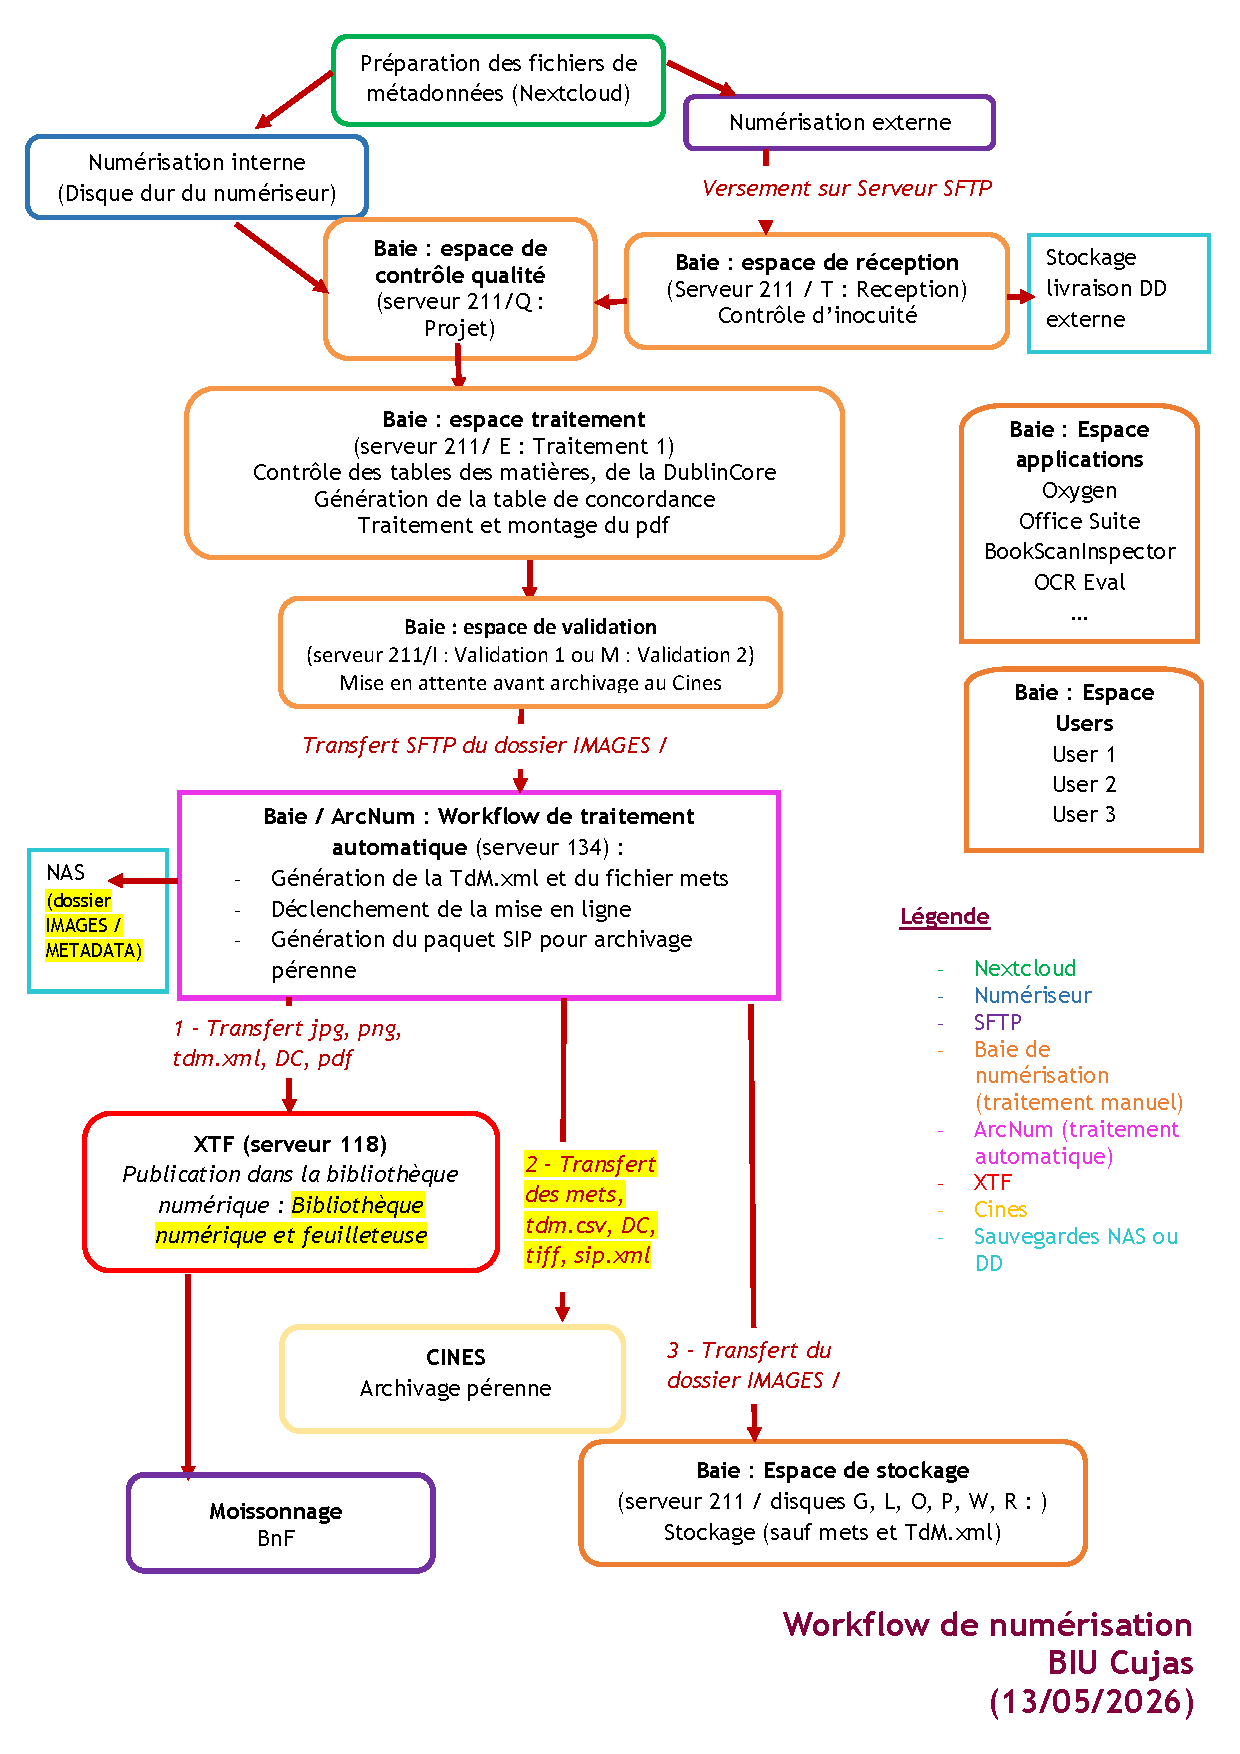
\includegraphics[width=0.5\linewidth]{202605_NUM_schemas_Workflow_prod_publ_V2.pdf}
		\caption{Schéma du workflow de production et de publication}
		\label{fig:workflow_prod_publ}
	\end{figure}

\subsection{Le matériel et le choix des chaînes de production (interne ou externe)}
La mise en œuvre concrète de cette chaîne de production a historiquement reposé sur l'acquisition d'un scanner de marque Kirtas à l'époque du projet Persée. Au-delà des arbitrages scientifiques, la mise en œuvre de la liste \enquote{Pfister-Roumy} se heurte rapidement aux contraintes matérielles de cet appareil. Cet équipement s'avère en effet beaucoup moins efficace que prévu, confrontant les agents à de \enquote{nombreux problèmes liés à son utilisation : il n'est pas possible d'utiliser toutes les fonctions automatiques de numérisation du scanner, forte probabilité de devoir passer en manuel pour les papiers anciens, difficultés de réglage et fréquents dysfonctionnements nécessitant d'éteindre et de rallumer les appareils et de refaire tous les réglages à chaque fois} \footcite{2007RefonteProgramme}. De surcroît, le scanner fait peser un fort risque de dégradation physique sur les documents originaux, dont la fragilité exige d'extrêmes précautions.

Malgré les difficultés logistiques pressenties face à l'ampleur d'un tel projet, l'établissement valide la liste \enquote{Pfister-Roumy} en articulant sa production autour d'une chaîne hybride. D'une part, à la suite de l'exposition virtuelle consacrée à Jean Carbonnier, la Bibliothèque Cujas dispose désormais d'une chaîne de numérisation en interne opérationnelle et prête à être mobilisée. Cette infrastructure s'est d'ailleurs renforcée grâce à la création de la célèbre \enquote{liste Pfister-Roumy}, une campagne de numérisation \enquote{alimentée entièrement en interne grâce aux compétences du département informatique} \footcite{2007RefonteProgramme}. Pour ce corpus, l'établissement fait le choix de traiter en interne exclusivement les \enquote{ouvrages postérieurs à 1830 avec l'océrisation et la relecture partielle sur les parties structurantes} \footcite{2007RefonteProgramme}. D'autre part, pour les documents antérieurs à 1830, la Bibliothèque Cujas privilégie une externalisation de la numérisation auprès d'un partenaire spécialisé, la société Puces et Plumes. Cette décision vise à \enquote{préserver le document}, car l'usage de son propre scanner représente un risque pour ces ouvrages déjà fragiles. Le prestataire se charge de numériser les documents en \enquote{mode image, [et] de faire la saisie fine des tables des matières} \footcite{2007RefonteProgramme}. Cette répartition stratégique du travail permet d'alimenter l'ambitieux projet de créer une bibliothèque numérique juridique fédérée unie par le protocole de moissonnage \ac{OAI-PMH}. Cette liste Pfister-Roumy constitue ainsi le véritable pilier fondateur de la bibliothèque numérique CujasNum.

Aujourd'hui, l'établissement dispose d'un nouveau matériel de numérisation de production récent (scanner de table de haute performance), ce qui permet de s'affranchir de ces contraintes historiques et de réévaluer la répartition entre traitements internes et externes. Le choix d'orienter un document vers la chaîne interne (numérisation sur place par les agents du \ac{DPCN}) ou vers une chaîne externe (prestataires ou chaînes de la \ac{BNF}) se fait désormais de manière stratégique par corpus, selon l'état de conservation physique de l'ouvrage, son format et les volumes à traiter.

\subsection{Le bordereau de numérisation}
Afin de garantir la bonne exécution de la campagne de numérisation, la méthodologie de travail de la Bibliothèque Cujas s'appuie sur l'établissement systématique d'un bordereau constituer de différentes parties. La première partie correspond à la notice bibliographique du document; la seconde détaille précisément sa pagination ainsi que les éventuelles particularités observées, par exemple des pages portant la même pagination; enfin, la dernière partie dresse l'état du document avant le transfert chez le prestataire \footannexe{\nameref{annexe_A_rapport_audit} pour voir l'entretien avec Sandrine Limandri qui détaille la façon dont la bibliothèque Cujas travail}.

\subsection{La phase de traitement: traitement d'images et OCRisation} 
Une fois la numérisation effectuée, la bibliothèque réceptionne les images brutes réalisées sous le format de conservation maître \ac{TIFF}. L'équipe effectue alors \enquote{un contrôle physique, livre en main, pour vérifier la complétude des images et s'assurer qu'aucune page ne manque par rapport au bordereau}\footannexe{\nameref{annexe_A_rapport_audit} pour voir l'entretien avec Sandrine Limandri.}. C'est par la suite qu'un script informatique local permet de générer les formats de diffusion légers (\ac{JPEG}, \ac{PDF}) et de produire automatiquement la table de concordance \enquote{qui fait correspondre chaque numéro d'image à la pagination réelle du livre}\footannexe{\ref{annexe_A_rapport_audit} pour voir l'entretien avec Sandrine Limandri.}. 

Cette orientation technique vers des fichiers statiques découle de la conception originelle de CujasNum, pensée comme \enquote{un simple répertoire \ac{PDF}} calqué sur la structure physique et matérielle d'un livre (volume et pages)\footannexe{\nameref{annexe_A_rapport_audit}.}. Pour dépasser cette contrainte et rendre la consultation des images plus ergonomique, une visionneuse \ac{JPEG} a été implémentée en 2013 pour permettre à l'usager de feuilleter le document de façon dynamique dans son navigateur\footannexe{\nameref{annexe_A_rapport_audit}.}.

\ac{XTF} possède de nombreuses contraintes techniques, l'une d'elles réside dans l'obligation d'avoir le format \ac{PDF} afin de mettre le document en ligne. Le système a été conçu comme \enquote{un simple répertoire \ac{PDF}} calqué sur la structure physique d'un livre (volume et pages)\footannexe{\nameref{annexe_A_rapport_audit}.}. Cela rend donc difficile l'ajout de tout autre types de documents ne respectant pas ce principe. Pour rendre la consultation des images plus agréable, une visionneuse \ac{JPEG} a été implémentée en 2013 pour permettre à l'usager de feuilleter le document de façon dynamique. 

Parallèlement au traitement de l'image, le traitement sémantique et textuel s'organise autour d'une stratégie d'océrisation (\ac{OCR}) différenciée. Au démarrage du traitement numérique, l'\ac{OCR} est appliqué exclusivement aux documents postérieurs à 1830 afin de permettre la recherche plein-texte au sein du texte imprimé\footcite{2011_programmeNumerisationPar}. Pour les ouvrages antérieurs à cette date charnière, la numérisation s'effectue uniquement en mode image pour préserver des supports physiques fragiles. L'absence d'\ac{OCR} sur le corpus de ces textes anciens est palliée par l'enrichissement sémantique de la table des matières, garantissant ainsi une navigation intellectuelle fine dans le document. Tandis que la personne en charge du contrôle qualité valide la conformité des métadonnées du Dublin Core, des moniteurs étudiants se voient confier la saisie intégrale de ces tables des matières sous format Excel/CSV, une tâche indispensable pour restituer fidèlement la structure de l'ouvrage et guider le chercheur\footannexe{\nameref{annexe_A_rapport_audit} pour voir l'entretien avec Sandrine Limandri.}.

\subsection{La phase de publication et d'archivage pérenne}
La validation définitive du contrôle qualité par l'équipe ouvre la voie à la phase finale de publication et d'archivage pérenne. Ce jalon requiert de minutieuses vérifications formelles et sémantiques effectuées par le technicien en charge de la validation. En plus de s'assurer de la conformité requise pour le versement au \ac{CINES}, le technicien doit \enquote{vérifier qu'il y a bien une image pour chaque page} et contrôler que le nommage de chaque fichier image respecte strictement la structure du \enquote{code-barres suivi du numéro d'image et de l'extension}\footannexe{\nameref{annexe_A_rapport_audit}.}. Il lui incombe également de s'assurer que les liens hypertextes figurant dans les métadonnées et commençant par le protocole non sécurisé \enquote{http} soient systématiquement remplacés par des adresses sécurisées \enquote{https} afin de prévenir tout blocage lors de l'ingestion ou de la consultation\footannexe{\nameref{annexe_A_rapport_audit}.}. 

Une fois ces critères formels validés, le protocole impose de contrôler la résolution et le taux de compression des images \ac{JPEG} et \ac{TIFF} à l'aide de l'outil \textit{IrfanView}, de verrouiller les fichiers \ac{PDF} de diffusion grâce à un mot de passe de protection institutionnel, et de valider la conformité de l'arborescence \ac{XML} du schéma de métadonnées Dublin Core afin de conjurer tout risque de rejet lors de l'ingestion par le \ac{CINES}\footcite{2010CRArchivage}. Les données sont ensuite transférées de manière asynchrone via un protocole \ac{SFTP} sécurisé (WinSCP) durant la nuit vers l'espace de publication final\footannexe{\nameref{annexe_A_rapport_audit} pour voir l'entretien avec Mebrouk Leulmi.}. Ce protocole de transfert différé, cloisonné et restreint a été mis en œuvre par le Département informatique technique (\ac{DIT}) à la suite d'une violente tentative d'attaque par rançongiciel subie par l'établissement en 2017, obligeant à sécuriser drastiquement tous les flux réseau entre la baie de traitement locale et les serveurs publics de l'université\footannexe{\nameref{annexe_A_rapport_audit} pour voir l'entretien avec Mebrouk Leulmi.}.

Le second volet de cette phase finale concerne l'archivage pérenne, confié au \ac{CINES}. Pour chaque ouvrage, la bibliothèque compile les fichiers d'images maîtres au format \ac{TIFF} et les fichiers de métadonnées descriptives et de gestion au format \ac{METS} (\textit{Metadata Encoding and Transmission Standard}) et PREMIS au sein d'un paquet de versement d'archives nommé \ac{SIP} (\textit{Submission Information Package})\footcite{2010CRArchivage}\footannexe{\nameref{annexe_A_rapport_audit} pour voir l'entretien avec Mebrouk Leulmi.}. Ce paquet standardisé garantit la préservation à long terme de la matière première numérique contre l'obsolescence matérielle. Néanmoins, ce circuit historique est aujourd'hui fragilisé. Le blocage récent des versements automatiques vers le \ac{CINES} contraint la Bibliothèque Cujas à conserver l'ensemble de ses fichiers intermédiaires au sein de son propre espace de stockage local (un \ac{NAS} de 40 à 50 téraoctets), provoquant une saturation critique de la baie de numérisation\footannexe{\nameref{annexe_A_rapport_audit}.}.

Cette procédure de versement réglementaire s'applique également aux documents dépourvus de structure linéaire, à l'instar du fonds iconographique de l'établissement. Pour répondre aux exigences d'ingestion du \ac{CINES}, les pièces d'images isolées doivent être compilées sous la forme d'un fichier \ac{PDF} unique. Le technicien élabore alors une table des matières et une table de concordance artificielles pour simuler la structure d'un volume physique, tandis qu'un plan d'archivage spécifique est défini conjointement avec les équipes du \ac{CINES} afin de valider ce profil de versement particulier\footannexe{\nameref{annexe_A_rapport_audit}.}.

Une autre particularité liée à la chaîne de numérisation réside dans l'indexation appliquée aux documents numériques de la bibliothèque numérique. C'est l'indexation Hauville qui est créée à partir de l'indexation \ac{RAMEAU}. 